\section{类型转换函数}
在介绍基本数据类型的时候,我们都提过它们之间的类型转换。比如说,一个 \lstinline@int@ 类型的数据可以转换成 \lstinline@double@ 型,反之亦然。我们可以用三种风格的语法来进行显式类型转换。就以 \lstinline@int@ 类型的 \lstinline@i@ 转换成 \lstinline@double@ 类型的 \lstinline@d@ 为例吧:
\begin{itemize}
    \item C风格类型转换:\lstinline@d=(double)i@
    \item 函数风格类型转换:\lstinline@d=double(i)@\footnote{注意,有些类型,比如 \lstinline@long long@ 或 \lstinline@int*@,如果想要通过函数风格进行类型转换,那么我们就要为这个类型套括号,写成 \lstinline@(long long)(i)@ 这样。}
    \item 静态类型转换:\lstinline@d=static_cast<double>(i)@
\end{itemize}\par
一般来说,在C++中我们更推荐使用静态类型转换,因为这个方法最稳妥。C风格方法在C++中是 \lstinline@const_cast@, \lstinline@reinterpret_cast@ 和 \lstinline@static_cast@ 的聚合。它在有些时候确实很方便,但是也能会因为太自由而带来我们不易发现的麻烦,所以我们需要加以限制。\par
至于函数风格的类型转换,这个更复杂些,这也是我们本节要讨论的重点。不过如果像我们刚才写的那样,一个圆括号里套单个数的话,它和C风格类型转换的效果是相同的。\par
\subsection*{转换构造函数}
我们可以用 \lstinline@double@ 类型来表示一个实数。虽然它的精度不够,不能表示真正意义上的无理数,但我们还是需要在精度上对它宽容一点的。\par
现在我不只想要表示实数,我还希望表示复数,那么我们就要写一个 \lstinline@Complex@ 类。它应当具备两个成员,一个表示实部,一个表示虚部,还支持一些简单的运算。
\begin{lstlisting}
class Complex {
private:
    double _r {}; //表示实部的值,默认初值为0
    double _i {}; //表示虚部的值,默认初值为0
public:
    Complex(double r, double i) : _r {r}, _i {i} {} //构造函数
    Complex(const Complex &c) : _r {c._r}, _i {c._i} {} //拷贝构造函数
    Complex& operator=(const Complex &c) { //赋值运算符
        _r = c._r;
        _i = c._i;
        return *this; //其实这里也不需要防止自我赋值,反正没风险
    }
    //...待补充
}; //这个Complex类不需要手动写析构函数,默认析构函数足够了
\end{lstlisting}
实数和复数之间有着密切的联系,我们能否让它们之间互相支持类型转换呢?我们的答案是``可以''!\par
在C++中,我们可以通过构造函数来实现其它类型到此类型的类型转换。我们把这种函数叫作\textbf{转换构造函数(Converting constructor)}。在转换构造函数当中最为特殊的,也就是传统意义上的转换构造函数,就是单个参数的转换构造函数\footnote{在C++11以前,只有单个参数的转换构造函数被认为是转换构造函数,其它的构造函数都不是。而在C++11以后,这个概念扩展到所有非 \lstinline@explicit@ 构造函数,但是单个参数的转换构造函数仍然是其中最常用的一种。本书也主要关注这一种。}。
\begin{lstlisting}
public:
    Complex(double r) : _r {r} {} //单个参数的转换构造函数
\end{lstlisting}
有了这个构造函数之后,我们就可以用前述三种风格的类型转换来把 \lstinline@double@ 类对象转换为 \lstinline@Complex@ 类对象了。\par
\begin{lstlisting}
void fun(Complex c) {} //什么也不做,单纯传个参
int main() {
    fun(0.); //把一个double对象传入fun函数?
}
\end{lstlisting}
事实证明这段代码是可以正常编译运行的——换句话说,\lstinline@double@ 类的 \lstinline@0.@ 被隐式类型转换成了 \lstinline@Complex@ 类的对象(按构造函数,这个个对象的实部和虚部都应当是 \lstinline@0.@),然后传入了 \lstinline@fun(Complex)@ 当中。\par
除了隐式类型转换,我们还可以写成如下显式的形式:
\begin{lstlisting}
    fun((Complex)0.); //C风格类型转换
    fun(Complex{0.}); //函数风格类型转换,使用花括号比圆括号更好
    fun(static_cast<Complex>(0.)); //静态类型转换
    fun(Complex{0.,0.}); //它可以接收两个参数,相当于对列表进行了类型转换
\end{lstlisting}\par
我们刚才是定义了两个构造函数对吧,其中一个用来接收单参数,一个用来接收双参数;除此之外我们还应当定义一个不接收参数的默认构造函数。这么多,有点太麻烦了。\par
为了简便起见,我们还可以把它改得更简洁一点,让一个构造函数代替这三个构造函数。读者可能猜到了,我们的方法就是设置默认参数:
\begin{lstlisting}
class Complex {
private:
    double _r {}; //表示实部的值,默认初值为0
    double _i {}; //表示虚部的值,默认初值为0
public:
    Complex(double r = {0}, double i = {0}) : _r{r}, _i{i} {}
    //带默认值的构造函数,可以接收零到二个参数
    Complex(const Complex &c) : _r {c._r}, _i {c._i} {} //拷贝构造函数
    Complex& operator=(const Complex &c) { //赋值运算符
        _r = c._r;
        _i = c._i;
        return *this; //其实这里也不需要防止自我赋值,反正没风险
    }
    //...待补充
};
\end{lstlisting}
在这种情况下我们也可以把它当作转换构造函数来用,效果相同,就请读者自行尝试吧。\par
类型转换的实际规则比我们想象中复杂很多。举个例子来说,如果你这样写,那也是可以通过编译的:
\begin{lstlisting}
    fun(0); //一个int型对象也能转换成Complex?
\end{lstlisting}
这里我们调用 \lstinline@fun@ 函数的时候传入的是 \lstinline@0@,这可是 \lstinline@int@ 型的对象啊!但是我们的构造函数中写的可是 \lstinline@double@,这怎么可能呢?\par
实际上,程序在运行时会先把 \lstinline@int@ 类型的 \lstinline@0@ 转换成 \lstinline@double@ 类型,然后再把 \lstinline@double@ 类型转换成 \lstinline@Complex@ 类型。所以一个看似云淡风轻的类型转换过程,其中会有多少复杂的细枝末节啊!\par
\subsection*{自定义转换函数}
构造函数能够部分地解决我们的类型转换需求,但不是全部。试想,我们可以通过 \lstinline@Complex::Complex(double={0}, double={0})@ 构造函数来实现 \lstinline@double@ 到 \lstinline@Complex@ 的类型转换,但是我们实现不了 \lstinline@Complex@ 到 \lstinline@double@ 的类型转换啊!我们总不可能写一个 \lstinline@double@ 的构造函数吧。\par
\textbf{自定义转换函数(User-defined conversion function)}能解决这个问题。它和转换构造函数相辅相成,转换构造函数规定了``哪些类型能转换成此类型'',而自定义转换函数则规定了``此类型能转换成哪些类型''。
\begin{figure}[htbp]
    \centering
    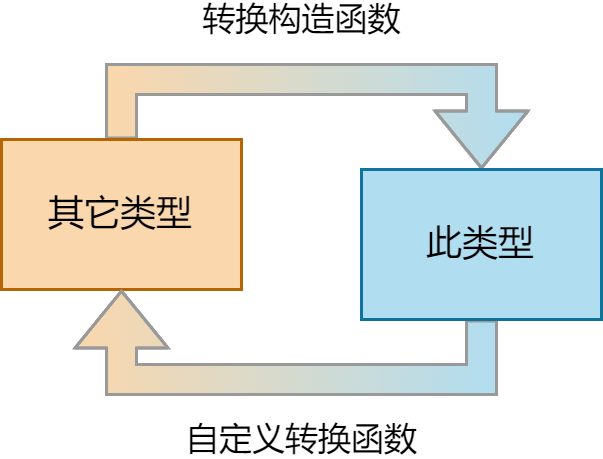
\includegraphics[width=0.6\textwidth]{../images/generalized_parts/08_type_conversion_between_classes_300.png}
    \caption{转换构造函数与自定义转换函数的作用}
\end{figure}
自定义转换函数的定义语法和运算符重载有点相似,不过又不尽相同。
\begin{lstlisting}
public:
    operator double() { //不允许指定返回类型,也不允许使用参数
        return _r; //这是类似截尾的处理方法,直接无视虚部,返回实部
    }
\end{lstlisting}
自定义转换函数不能指定返回类型,看上去和构造函数有点像,但它们根本不一样!构造函数是``没有返回值'',我们调用构造函数之前这个对象已经存在;而自定义转换函数其实有返回值,只不过它的返回类型是写在了函数名中,所以我们不用单拎出来再写一次。\par
自定义转换函数也不能指定参数,这是因为转换函数只能接收一个参数——没错,正是我们反复提及的那个``调用它的函数''。在实际的类型转换过程中,我们的确可以写成 \lstinline@c.operator double()@,不过我们很少这个干,而是用那三种常见的类型转换语法。
\begin{lstlisting}
    Complex c{1,2};
    std::cout << (double)c << std::endl; //C风格转换
    std::cout << double{c} << std::endl; //函数风格类型转换,这里也用花括号
    std::cout << static_cast<double>(c) << std::endl; //静态类型转换
    std::cout << c.operator double(); //客串一下而已,完全不推荐使用
\end{lstlisting}\par
最后我们来尝试一个更有趣的例子:为 \lstinline@valarri@ 设计一个转换构造函数和一个自定义转换函数,允许我们把 \lstinline@valarri@ 对象转换成 \lstinline@std::vector<int>@ 对象,反之亦然。\par
为了方便起见,我们还是使用 \lstinline@vecint@ 作为 \lstinline@std::vector<int>@ 的别名,但其中道理是不变的。
\begin{lstlisting}
#include <vector> //使用vector必备的库
using vecint = std::vector<int>; //别名声明
\end{lstlisting}
接下来我们先考虑它们的声明:
\begin{lstlisting}
//声明
public:
    valarri(const vecint&); //vecint到valarri的转换构造函数
    operator vecint()const; //valarri到vecint的自定义转换函数
\end{lstlisting}
我们的转换构造函数应设为 \lstinline@const vecint&@,这样的好处是它可以接收常量作为参数——常量对象当然也可以类型转换嘛。同样的道理,我们也应该把自定义转换函数设为常成员函数。\par
在定义其转换构造函数时,不要忘记定义构造函数的一般规则——初值列和默认成员初始值,代码重用等。如果你有计数器,也别忘了这个静态成员。
\begin{lstlisting}
valarri::valarri(const vecint &vec) //vecint到valarri的转换构造函数
    : _cap {vec.size()}, //valarri的成员对vec私有成员无访问权限,要用其公有成员
    _size {vec.size()}
{
    for (int i = 0; i < _size; i++)
        operator[](i) = vec[i]; //vecint也有重载下标运算符,且有常成员函数的重载
    _object_number++; //计数器自增
}
\end{lstlisting}
这里的 \lstinline@operator[](i)@ 用法有点特别,我来解释一下。\par
我们在前面已经定义了两个 \lstinline@valarri@ 的下标运算符重载,一个是常成员函数,另一个不是。
\begin{lstlisting}
public:
    int& operator[](int i) { return _arr.p()[i]; } //下标,非常成员函数
    int operator[](int i)const { return _arr.p()[i]; } //下标,常成员函数
\end{lstlisting}
所以我们当然也可以调用这个成员函数了。这个成员函数的函数名是 \lstinline@operator[]@,接收一个 \lstinline@int@ 型参数,所以我们调用时就要写成 \lstinline@operator[](i)@,这就合理了吧。\par
如果你认为这种写法太过奇怪,不能接收,那么你也可以写成 \lstinline@(*this)[i]@。\lstinline@this@ 是指向本对象的指针,那么 \lstinline@(*this)@ 就是本对象;而 \lstinline@(*this)[i]@ 就是本对象在调用下标运算符嘛,这就很好理解了。\par
至于自定义转换函数,它的道理是一样的,我就不加讲解直接写了。
\begin{lstlisting}
valarri::operator vecint()const { //valarri到vecint的自定义转换函数
    vecint vec(_size); //调用了vecint的构造函数,直接指定vec的大小
    for (int i = 0; i < _size; i++)
        vec[i] = operator[](i); //逐个赋值,不要用push_back,反复重分配太费时
    return vec;
}
\end{lstlisting}
这里我们调用 \lstinline@vecint@ 的构造函数时依然要注意,要用圆括号而不是方括号。\par
有了这个类型转换函数之后,对于期待 \lstinline@vecint@ 的场合,我们也可以用 \lstinline@valarri@ 通过类型转换来传入参数;反之亦然。这样一来,我们就能可以在一定程度上打破这两个类型的隔绝状况。\par
\subsection*{隐式类型转换与函数重载}
有的时候用隐式类型转换可以帮助我们节省很多运算符/函数重载方面的压力。就以复数类而言吧,如果我们需要重载加法运算符,可能我们需要这些函数:
\begin{lstlisting}
Complex Complex::operator+(const Complex &com)const; //成员函数
Complex Complex::operator+(double num)const; //成员函数
Complex operator+(double num, const Complex com); //非成员函数
\end{lstlisting}
这三种情况分别对应着复数+复数/复数+实数/实数+复数。看上去真是又麻烦,又杂乱——我们还要为减法/乘法/除法等,对每个运算符都要定义三个版本才行。\par
但是有了类型转换之后,我们只需要定义单个版本就够了:
\begin{lstlisting}
Complex Complex::Complex(double r, double i); //转换构造函数,其中i可以有默认值
Complex operator+(const Complex &com1, const Complex &com2); //只此一个足够了
\end{lstlisting}
那么,在遇到复数加实数或者实数加复数的情况时会发生什么呢?答案是:传入的实数会隐式类型转换成复数。
\begin{lstlisting}
    Complex{1,2} + 1.5; //(1+2i)+1.5
\end{lstlisting}
在这里,\lstinline@Complex{1,2}@ 不是``构造函数的返回值'',因为构造函数是没有返回值的。这个语法的正确解读应为:\lstinline@Complex(1,2)@ 是构造函数创建的临时对象,这和 \lstinline@int@ 转换成 \lstinline@double@ 过程中创建了一个临时数据是同样的道理。\par
至于 \lstinline@1.5@,它也会不动声色地隐式类型转换为 \lstinline@Complex{1.5,0}@,于是我们不需要为了 \lstinline@Complex+double@ 专门写一个运算符重载,只需要让它自己隐式类型转换就够了。\par
\subsection*{\texttt{explicit}}
隐式类型转换虽然方便,但是未必总能合我们的意。有些时候,隐式类型转换不能满足我们的需要,所以我们需要显式类型转换。比如说,当我们试图用 \lstinline@std::cout@ 输出一个 \lstinline@char*@ 指针的值时,实际的输出是一个字符串。为了输出地址值,我们应当用显式类型转换来实现:
\begin{lstlisting}
    char *pch = nullptr;
    std::cout << static_cast<void*>(pch); //显式类型转换为void*
\end{lstlisting}\par
还有些时候,一些我们本来不想进行,但却被编译器自动执行的隐式类型转换可能会引发出乎意料的错误。在不久前我们就看过了一个这样的例子:
\begin{lstlisting}
    std::string str3 {33, '='}; //试图通过统一初始化调用(size_type, CharT)版本
    std::cout << str3; //但输出的内容却是!=
\end{lstlisting}
这是因为,\lstinline@int@ 类型的 \lstinline@33@ 在这里被隐式类型转换成了 \lstinline@char@ 类型的 \lstinline@'!'@,然后与这里的 \lstinline@'='@ 一并构成 \lstinline@std::initializer_list<char>@。于是实际调用的是这个构造函数\footnote{此处的 \lstinline@CharT@ 正是 \lstinline@char@,\lstinline@size_type@ 正是 \lstinline@std::size_t@,读者可以用 \lstinline@std::is_same@ 验证之。}:
\begin{lstlisting}
basic_string(
    std::initializer_list<CharT> ilist,
    const Allocator& alloc = Allocator()
); //接收一个std::initializer_liist<CharT>参数
\end{lstlisting}
然而我们的本意是调用这个构造函数:
\begin{lstlisting}
basic_string(
    size_type count,
    CharT ch,
    const Allocator& alloc = Allocator()
);
\end{lstlisting}\par
回到这个问题本身,我们发现它的根源就在于:\textbf{在编译的过程中,编译器选择了我们意料之外的隐式类型转换方案}。这是隐式类型转换的一个致命缺点。\par
我们在写复数类的时候也可能遭遇类似的情境,我们不想进行某种类型转换,但编译器却自动进行了隐式类型转换。为了防止隐式类型转换的发生,同时又保留类型转换的功能,我们可以使用关键字 \lstinline@explicit@。\par
\lstinline@explicit@ 说明符的作用在于,限制某种类型转换必须以显式类型转换(Explicit type conversion)的方式进行。如果我们想设计一个 \lstinline@valarri@ 向 \lstinline@bool@ 的转换函数,用 \lstinline@true@/\lstinline@false@ 来表示这个 \lstinline@valarri@ 中是否有数据,那么我们可以这样写:
\begin{lstlisting}
//声明&定义
public:
    explicit operator bool()const { return _size; }
    //valarri到bool的自定义转换函数,说明此数组中是否有数据,是常成员函数
\end{lstlisting}\par
读者需要搞清楚 \lstinline@explicit@ 的作用。它的作用不是``规定在这个函数中不能隐式类型转换''或者``这个类不能隐式类型转换''等等——这些都不对。它的作用是:规定了 \lstinline@valarri@ 到 \lstinline@bool@ 的类型转换过程必须显式。至于其它的任何类型转换过程,都不受此影响。\par
比如说吧,我们在函数体内就返回了一个 \lstinline@std::size_t@ 类型的 \lstinline@_size@,但是期待的返回类型是 \lstinline@bool@,这时会发生什么呢?\lstinline@_size@ 会被隐式类型转换为 \lstinline@bool@\footnote{在转换过程中,\lstinline@std::size_t{0}@ 会被转换为 \lstinline@false@,其它值一律被转换为 \lstinline@true@},然后作为返回值。所以说,声明为 \lstinline@explicit@ 的函数内部仍然可以进行其它类型之间的类型转换,这是不受 \lstinline@explicit@ 影响的。\par
如果我们要使用这个类型转换函数,就必须显式类型转换,或者用于条件、循环结构的判断句,或者用于逻辑表达式\footnote{在条件和循环结构中,比如 \lstinline@if(std::cin)@,虽然这里发生的也是隐式类型转换,但编译器是允许的,因为这里发生的隐式类型转换不会有任何二义性的可能。同理,逻辑运算符 \lstinline@&&@, \lstinline@||@ 和 \lstinline@!@(特指内置的运算符,而不是用户重载的)在接收操作数时也可以发生隐式类型转换,这种隐式类型转换是允许的。总之,\lstinline@explicit@ 的限制范围是个很复杂的问题。}。
\begin{lstlisting}
void fun(bool) {}
int main() {
    valarri arr{};
    valarri a; //将调用默认构造函数
    if (!a) //a没有重载!运算符,所以内置!运算符会期待a转换成bool类型
        std::cout << bool(a); //可以进行显式类型转换
    if (a) //if期待a转换成bool类型,这里可以转换
        fun(a); //试图在参数传递时使用隐式类型转换
//error: cannot convert 'valarri' to 'bool'
}
\end{lstlisting}
\subsection*{\texttt{valarri}的初步实现代码}
最后,我们可以把前五节已有的知识串联起来,完善一下我们的 \lstinline@valarri@ 代码。\par
下面是我修改完善过后的完整代码,只有头文件和定义部分。读者可以自行写一个主函数并测试其主要功能。\par
相比于之前断断续续写的代码,这里的内容更详细,更具体,改动了部分代码(比如,在构造函数中添加 \lstinline@size@ 超过 \lstinline@MAX_SIZE@ 的检测,把循环变量改成统一的 \lstinline@std::size_t@ 类,还把依靠 \lstinline@_arr.p()[]@ 成员实现的部分用 \lstinline@operator[]()@ 实现),新增了 \lstinline@resize@ 和 \lstinline@swap@ 成员函数,对注释部分也做了相当大的调整。
\lstinputlisting[caption=\texttt{Header.h}]{../code_in_book/8.1-8.2/Header.h}
\lstinputlisting[caption=\texttt{Definition.cpp}]{../code_in_book/8.1-8.2/Definition.cpp}
